% Ubah kalimat sesuai dengan judul dari bab ini
\chapter{TINJAUAN PUSTAKA}

% Ubah konten-konten berikut sesuai dengan yang ingin diisi pada bab ini

\section{Roket Luar Angkasa}

% Contoh input gambar dengan format *.jpg
\begin{figure} [ht] \centering
  % Nama dari file gambar yang diinputkan
  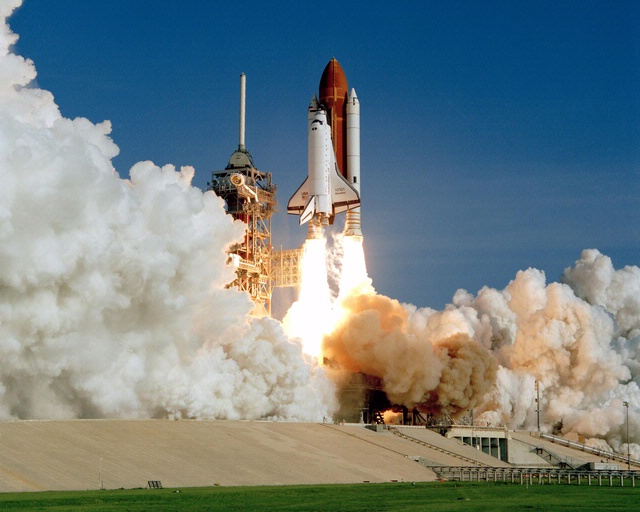
\includegraphics[scale=0.3]{gambar/space-shuttle.jpg}
  % Keterangan gambar yang diinputkan
  \caption{Peluncuran pesawat luar angkasa Discovery \citep{DiscoverySpaceShuttle}}
  % Label referensi dari gambar yang diinputkan
  \label{fig:SpaceShuttle}
\end{figure}

Roket luar angkasa merupakan \lipsum[16][1-10]

% Contoh penggunaan referensi dari gambar yang diinputkan
\emph{Discovery}, Gambar \ref{fig:SpaceShuttle}, merupakan \lipsum[17][1-9]

\section{Gravitasi}

Gravitasi merupakan \lipsum[18][1-10]

\subsection{Hukum Newton}

% Contoh penggunaan referensi dari pustaka
Newton \citep{Newton1687} pernah merumuskan bahwa \lipsum[19]
% Contoh penggunaan referensi dari persamaan
Kemudian menjadi persamaan seperti pada persamaan \ref{eq:FirstNewtonLaw}.

% Contoh pembuatan persamaan
\begin{equation}
  % Label referensi dari persamaan yang dibuat
  \label{eq:FirstNewtonLaw}
  % Baris kode persamaan yang dibuat
  \sum \mathbf{F} = 0\; \Leftrightarrow\; \frac{\mathrm{d} \mathbf{v} }{\mathrm{d}t} = 0.
\end{equation}

\subsection{Anti Gravitasi}

Anti gravitasi merupakan \lipsum[20]
